\documentclass{article}
\usepackage{geometry}
\usepackage{listings}
\usepackage{color}
\usepackage{hyperref}
\usepackage{listings}
\usepackage{graphicx}
\usepackage{float}
\usepackage{sectsty}
\usepackage{enumitem}

\definecolor{codebackground}{rgb}{0.99,0.99,0.97}
\definecolor{mygray}{rgb}{0.5,0.5,0.5}

\lstset{
    basicstyle=\ttfamily,
    backgroundcolor=\color{white},
    keywordstyle=\color{blue},
    commentstyle=\color{mygray},
    showstringspaces=false,
    numbers=left,
    numberstyle=\tiny,
    numbersep=5pt,
    breaklines=true,
    frame=single,
    breakatwhitespace=false,
}

\geometry{a4paper, margin=0.75in}

\title{\textbf{CS3510 - Operating System}\\Assignment 2}
\author{\textbf{Soham Rajesh Pawar}\\CS22BTECH11055}
\date{November 27, 2023}

\begin{document}
\maketitle

\section{Coding Approach :}
{\large The program was implemented in C to find the vampire numbers in the range 1 to \texttt{N}(obtained from the input file) by dividing the task among \texttt{K} threads.}
\\
\subsection{Steps :}
\begin{enumerate}
\item{First we read \texttt{N} and \texttt{K} from the input file.}
\item{The main process creates \texttt{K} threads, each of which will execute a common routine.}
\item{According to the routine each thread will check the numberset it has been allotted to get the vampire numbers in the concerned set.}
\begin{enumerate}
\item{The allottment of numbers is decided using the thread id which is passed as a routine parameter(the counter variable i). Each number that is i (mod \texttt{K}) will be allotted to thread i + 1.}
\item{To check if a number is Vampire or not, we will iterate through it's factors and check each pair of factors individually.}
\end{enumerate}
\item{If a thread identifies a pair of fangs for a number in it's set then it will record the number identified in the common log file along with it's own identity.}
\item{The main process waits for the completion of all threads and collects the resources.}
\end{enumerate}
\section{Verification :}
{\large The main log file aka OutFile.log also contains the count of vampire numbers within the given range and the time required for the execution of the task for verification purposes.}
\section{Conclusion :}
{\large
\begin{enumerate}
\item{Increasing the input size naturally increases the execution time.}
\item{Increase in the number of processes generally leads to a decrease in execution time. However, after a certain number increasing the number of processes grants diminishing returns. This could possibly be due to the distribution of vampire numbers among the natural numbers.}
\section{Graphs :}
\subsection{Maintaining \texttt{K} at 8\\Time vs Size(2^{N}) :}
\begin{figure}[H]
  \centering
  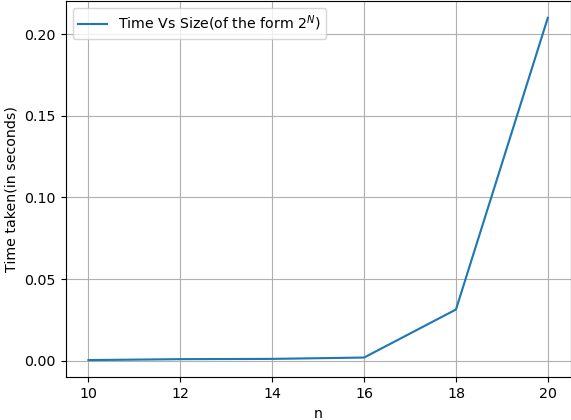
\includegraphics[width=0.8\linewidth]{1.png}
  \label{fig:your_label}
\end{figure}
\subsection{Maintaining Size at 10,00,000\\Time vs Number of Processes(\texttt{K}) :}
\begin{figure}[H]
  \centering
  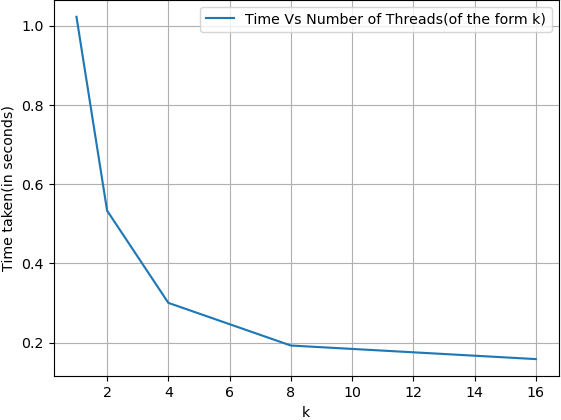
\includegraphics[width=0.8\linewidth]{2.png}
  \label{fig:your_label}
\end{figure}
\end{document}
